%This is an explanation of how we constructed our different feature vectors which we later used to try our algorithms.
%\\\\
The documents were processed in the following order:
\begin{enumerate}
\item Filter out unwanted characters as: . , ? , ! etc.
\item Remove stop-words as: and, or, this etc.
\item Optionally: make use of Snowball, a stemmer which removes endings of
words \citep{snowball_url}.
\item Either use unigram or bigram as elements to the feature vector
\item Make use of TF–IDF, term frequency–inverse document frequency that
reflects on how important a word is to a document in a collection or corpus
\item Choose the feature size, meaning the number of most common words to use
 in the classification.
\end{enumerate}
Each document was assigned a label corresponding to its sentimentality
(positive or negative) and another label corresponding to its topic.
All processed data were stored in different Matlab binary files depending on the
different feature selections.
\\\\
The generated feature vector using bigrams differed a lot from the one using
unigram. It appeard as the bigrams were to unique and each bigram was only
present in a small number of documents, making it hard to classify.  This is
shown in Figure~\ref{fig:docperfeature}. The maximum number of documents that contain a certain feature is for unigrams 2941 documents and for bigram 106 documents.
\begin{figure}[h!]
\centering
        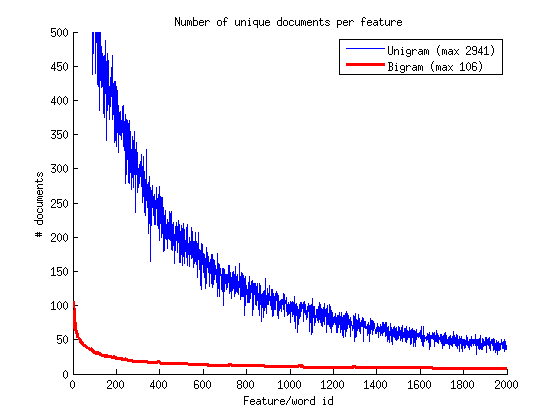
\includegraphics[scale = 0.6]{../Plottar/documents_per_feature.png}
\caption{Number of documents that contain a certain feature}
\label{fig:docperfeature}
\end{figure}
%Feature values corresponds to the term occurrence frequencies.
%The calculation for this was done in a number of steps.

%The text categorization was implemented in python. Feature values was generated
%for both 1-grams and 2-grams to be able to see if a n-gram, $n > 1$, improves
%the result when running the classification algorithms.

%The output data is represented by a matrix $(words \times document)$ where each
%elements represents the TF-IDF value for the frequency of a word in a specific
%document.
%It's obvious for one to realize that it isn't possible to take all unique words
%into account since the output matrix would have been enormous if so was the
%case. Even further it's not obvious that the classification results gets better
%just because every word is taken into account. Therefor several tests was
%performed using different number of features or more specific words or bigrams
%in this case.
